\documentclass[conference]{IEEEtran}
% \IEEEoverridecommandlockouts
% The preceding line is only needed to identify funding in the first footnote. If that is unneeded, please comment it out.
\usepackage{cite}
\usepackage{amsmath,amssymb,amsfonts,mathtools,tikz}
\usepackage{algorithmic}
\usepackage{graphicx}
\usepackage{textcomp}
\usepackage{xcolor}
\usetikzlibrary{shapes,arrows,positioning}
\def\BibTeX{{\rm B\kern-.05em{\sc i\kern-.025em b}\kern-.08em
    T\kern-.1667em\lower.7ex\hbox{E}\kern-.125emX}}
\begin{document}

\title{Information-Optimizing Control of Multi-Agent Systems\\
{\footnotesize 16.32: Principles of Optimal Control and Estimation Term Project}}

\author{\IEEEauthorblockN{Eyassu B. Shimelis}
Cambridge, Massachusetts \\
eyassu.shimelis@ll.mit.edu \\
}

% Definition of blocks:
\tikzset{%
  block/.style    = {draw, thick, rectangle, minimum height = 3em,
    minimum width = 3em},
  sum/.style      = {draw, circle, node distance = 2cm}, % Adder
  input/.style    = {coordinate}, % Input
  output/.style   = {coordinate} % Output
}
% Defining string as labels of certain blocks.
\newcommand{\suma}{\Large$+$}
\newcommand{\inte}{$\displaystyle \int$}
\newcommand{\derv}{\huge$\frac{d}{dt}$}


\maketitle
\thispagestyle{plain}
\pagestyle{plain}

\begin{abstract}
This report describes the implementation and results of using GPOPS-II to determine locally-optimal solutions for multi-agent path planning. The problem is formulated as a numerical optimization over space and time, with the goal of maximizing the position information of a primary agent. The solution is computed jointly; that is, an augmented state vector containing the states of all agents. The goal is to escort an autonomoous agent across an obstacle-filled map, while minimizing the time and expended control effort. With an adequate initial guess, GPOPS-II is able to find an optimal solution for all agents in a reasonable time (approx. 10 min) for four agents and five obstacles. This method, however, is not ideal for larger problems due to scaling issues, which are discussed in this report.
\end{abstract}

\section{Introduction}
In a classical sense, estimation is incorporated into control systems in order to improve their performance, when they are subject to noise. For example, in certain linear cases, Linear-quadratic-Gaussian (LQG) control is an example of how the two work together, seamlessly and optimally.

This project is motivated by nonlinear, estimatiors that may be aided by information-maximizing control. Examples of this include remote sensing and collaborative robotics. Here, the primary performance metric may be the results of the estimator and not the control.

\section{Problem Formulation}
\subsection{Autonomous Convoy}
This report considers a toy example: one of an autonomous convoy with two types of sensors. Each agent has a global positioning sensor and a relative range sensor. The GPS allows the agent to accurately estimate its global position in the map. The relative range sensor (e.g. sonar, received signal strength indicator, ultrawideband) measures the relative distance between two agents.

Despite the simplicity of the problem, it motivates many interesting research questions in estimation and control. For example, previous work \cite{florian} has demonstrated a method of multi-agent estimation in a distributed manner. The authors demonstrate unique algorithms for performing approximate inference on the complex factor graphs, which arise from the relative measurements between agents. Other work \cite{spletzer} has looked into complex and clever control strategies, which result in improved localization in imagery-based, cooperative localization.

\begin{figure}[h!]
\begin{center}
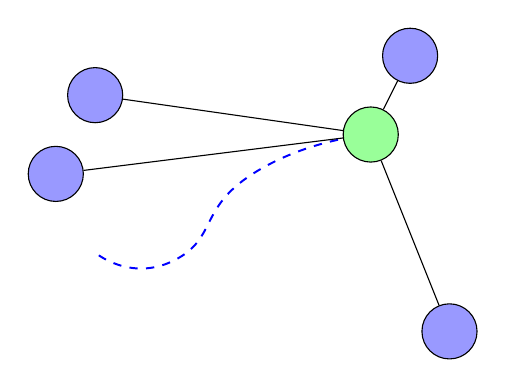
\begin{tikzpicture}[auto, node distance=1cm,>=latex']
\draw [cyan, line width=0.25mm, dashed, color=blue] plot [smooth, tension=1] coordinates { (2.5,1.5) (1,1) (0,-0.1) (-1, 0)};

\node[circle,draw, minimum size=0.7cm, fill=green!40!white] (A) at  (2.5,1.5)  {};

\node[circle,draw, minimum size=0.7cm, fill=blue!40!white] (B) at  (3.5,-1) {};
\node[circle,draw, minimum size=0.7cm, fill=blue!40!white] (C) at  (-1,2) {};
\node[circle,draw, minimum size=0.7cm, fill=blue!40!white] (D) at  (3,2.5) {};
\node[circle,draw, minimum size=0.7cm, fill=blue!40!white] (E) at  (-1.5,1) {};

\draw (A) -- (B);
\draw (A) -- (C);
\draw (A) -- (D);
\draw (A) -- (E);

\end{tikzpicture}
\end{center}
\caption{Autonomous convoy of multi-agent system. The secondary agents (blue) are well localized, but the primary agent (green) must rely on relative range measurements to localize itself.}
\label{convoy}
\end{figure}


\subsection{Geometric Dilution of Precision}
There are many systems out in the world which attempt to estimate position from relative range measuremts. An example of this is the Global Positioning System (GPS). A GPS receiver is able to estimate its position using the signal time-of-arrival (TOA) and positions of a subset of time-synchronized satellites. The quality of this position estimate is related to the geometric diversity of the transmitters. 

The sensitivty of the estimated state to the transmitter spatial configuration is surmised by the Geometric Dilution of Precision (GDOP). More precisely, the GDOP is a single-valued function $g: \mathbb{R}^{N \times M} \to \mathbb{R}$, where $N$ is the number of agents and $M$ is the dimensionality of each agent's position.

The GDOP can be explained graphically. For example, Fig. \ref{bad_gdop} shows two transmitters are close to each other. In cases like this, small errors in the measured range may result in significant differences in inferred position. On the other hand, when the transmitters are spread out, the intersection of their noisy measurements reults in a smaller position-error patch. That is, the sensitivity of measurement errors is reduced, as shown in Fig. \ref{good_gdop}.

\begin{figure}[h!]
\begin{center}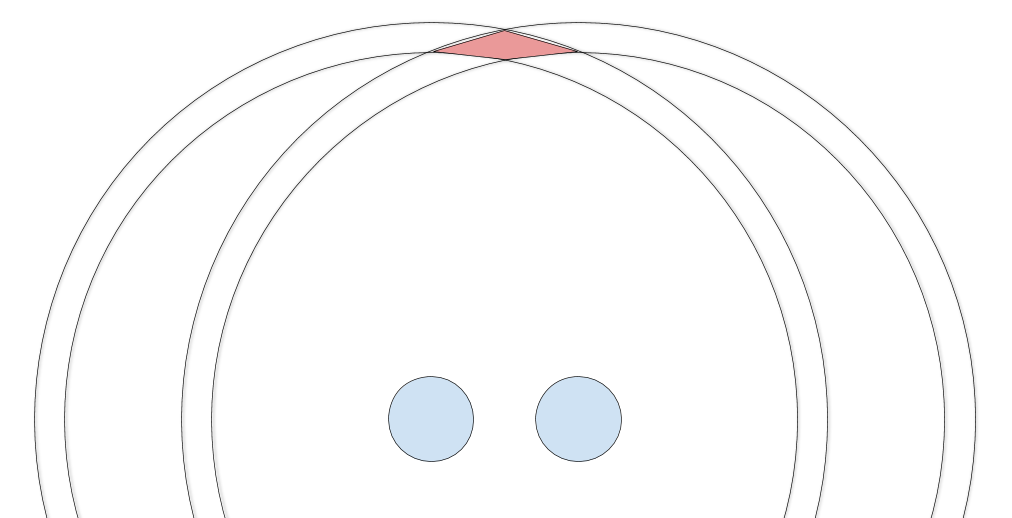
\includegraphics[width=0.3\textwidth]{img/bad_gdop.png}
\caption{Example of poor spatial diversity of transmitters. Results in a high dilution of precision.}
\label{bad_gdop}
\end{center}
\end{figure}

\begin{figure}[h!]
\begin{center}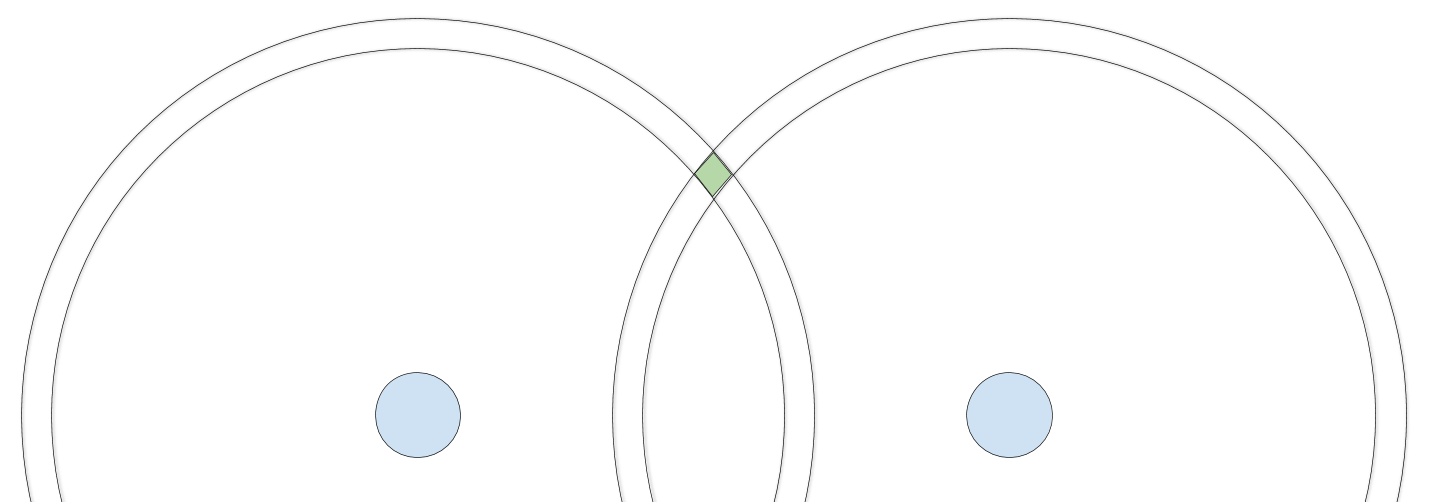
\includegraphics[width=0.4\textwidth]{img/good_gdop.png}
\caption{Example of good spatial diversity of transmitters. Resulting in a low dilution of precision.}
\label{good_gdop}
\end{center}
\end{figure}

For $N-1$ transmitters and one receiver--in two dimenstions--the GDOP is calculated by first constructing a matrix of unit vectors.
\begin{align}
A &= \begin{bmatrix} \frac{x_1 - x}{R_1} & \frac{y_1 - y}{R_1} & 1 \\ & \vdots & \\ \frac{x_N - x}{R_N} & \frac{y_N - y}{R_N} & 1 \\ \end{bmatrix} \\
\intertext{The GDOP is then calculated as}
\text{GDOP} &= \sqrt{tr \{ \left( A^T A\right) ^{-1} \}}
\end{align}

Note: GDOP is a convenient proxy for information, as we have posed the problem. It assigns a numeric value to the quality of a geometric configuration\cite{gdop}.

\subsection{Optimization Problem Formulation}
The next step is to formulate the problem as an optimal control problem. We seek to find an optimal path through an obstacle-filled map, while minimizing the GDOP. Additionally, we want the solution to be minimum-time and minimum-fuel. Begin by defining the objective function, which is a weighted sum of these metrics.
\[ \phi(x(t), ~u(t),~t) = \int_{t_0}^{tf} R_t t + R_{u}u^2 + R_{g} g(x(t))\]

The goal is to minimize the objective funtion
\begin{align}
J &= \phi (x(t),~u(t),~t), \\
\intertext{subject to dynamic constraints}
\dot{x} &= Ax + u\\
\intertext{and path constraints}
0 &\geq c(x(t),~u(t),~t).
\end{align}

\subsection{State Dynamics and Constraints}
For this problem, the agent's state consists of their position and velocity. They can control their position by independently applying a force in the x- or y-direction. To compute a joint solution, the agent's states were concatenated into a augmented single vector. The linear state dynamics are shown below:

\[ \begin{bmatrix} \dot{x}_1 \\ \dot{y}_1 \\ \ddot{x}_1 \\ \ddot{y}_1 \\ \vdots \\ \dot{x}_n \\ \dot{y}_n \\ \ddot{x}_n \\ \ddot{y}_n \end{bmatrix}= \begin{bmatrix} 0 & 0 & 1 & 0 \\ 0 & 0 & 0 & 1 & \dots \\ 0 & 0 & 0 & 0 \\ 0 & 0 & 0 & 0 \\ &\vdots & & &  \ddots \\ & & & & & 0 & 0 & 1 & 0 \\ & & & & & 0 & 0 & 0 & 1 \\& & & & &  0 & 0 & 0 & 0 \\& & & & &  0 & 0 & 0 & 0 \end{bmatrix} \begin{bmatrix} x_1 \\ y_1 \\ \dot{x}_1 \\ \dot{y}_1 \\ \vdots \\ x_n \\ y_n \\ \dot{x}_n \\ \dot{y}_n \end{bmatrix} + \begin{bmatrix} 0 \\ 0 \\ u_{x_1} \\ u_{y_1} \\ \vdots \\ 0 \\ 0 \\ u_{x_n} \\ u_{y_n}\end{bmatrix}\]

For some realism, the control for each agent is limited.
\[ |u| \leq u_{\text{max}} \]

Additionally, the secondary agents are constrained to remain within a maximum distance from the primary agent. 
\[ d(t) \leq r_{\text{max}} \]

This was added to enforce a maximum measurement/communication range between agents. And finally, agent paths may not intersect any obstacles.
\[ x(t) \cap O \leq 0\]

Fig. \ref{map} shows an example of the maps used in the optimization problem.
\begin{figure}[h!]
\begin{center}
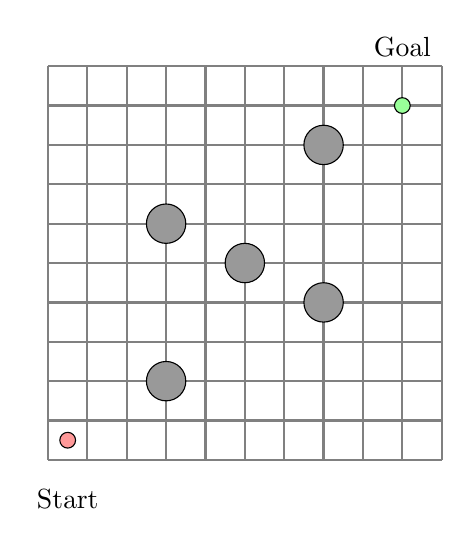
\begin{tikzpicture}[auto, node distance=1cm,>=latex']
\draw (0, 0) -- (5, 0) -- (5, 5) -- (0,5) -- (0, 0);
\draw[step=0.5,gray,thick] (0,0) grid (5,5);

% obstacles
\draw[black,fill=black!40!white] (1.5, 1) circle (0.25);
\draw[black,fill=black!40!white] (3.5, 2) circle (0.25);
\draw[black,fill=black!40!white] (1.5, 3) circle (0.25);
\draw[black,fill=black!40!white] (3.5, 4) circle (0.25);
\draw[black,fill=black!40!white] (2.5, 2.5) circle (0.25);

\draw[black,fill=red!40!white] (0.25, 0.25) circle (0.1);
\node[align=center] at (0.25, -0.5) {Start};

\draw[black,fill=green!40!white] (4.5, 4.5) circle (0.1);
\node[align=left] at (4.5, 5.25) {Goal};

\end{tikzpicture}
\caption{Example of a map. The red and green points denote the start and goal, respectively. The gray points indicate obstacles that the final paths may not intersect.}
\label{map}
\end{center}
\end{figure}

\subsection{Implementation}
This optimal control problem was written using the GPOPS-II library. GPOPS-II is a general purpose optimal control library, written in MATLAB\cite{gpops}. It is able to solve complex optimization problems by approximating them using nonlinear programming techniques. The NLP translation is done under the hood, and relies on variable-order Gaussian quadrature methods.

For this problem, the GPOPS-II code was parameterized to accept a variable number of agents, obstacles, obstacle configurations, start regions, and goal regions.

\subsection{Technical Considerations and Assumptions}
The problem was initially planned to work with rectangular obstacles. For simplicity, this was converted to using circles, since it is easier to write a smooth function for numerically describing intersection (i.e. distance to obstacle origin minus obstacle radius). 

\section{Results}
For well-conditioned problems, GPOPS-II converges to an optimal solution within a dozen minutes. Below are two results from two of these runs. The obstacles between the two runs are varied.

The top left subplot of figures \ref{results_1} and \ref{results_2} show an overhead path of the agents, with other components of the state in the remaining subplots.

\begin{figure*}[h!]
\begin{center}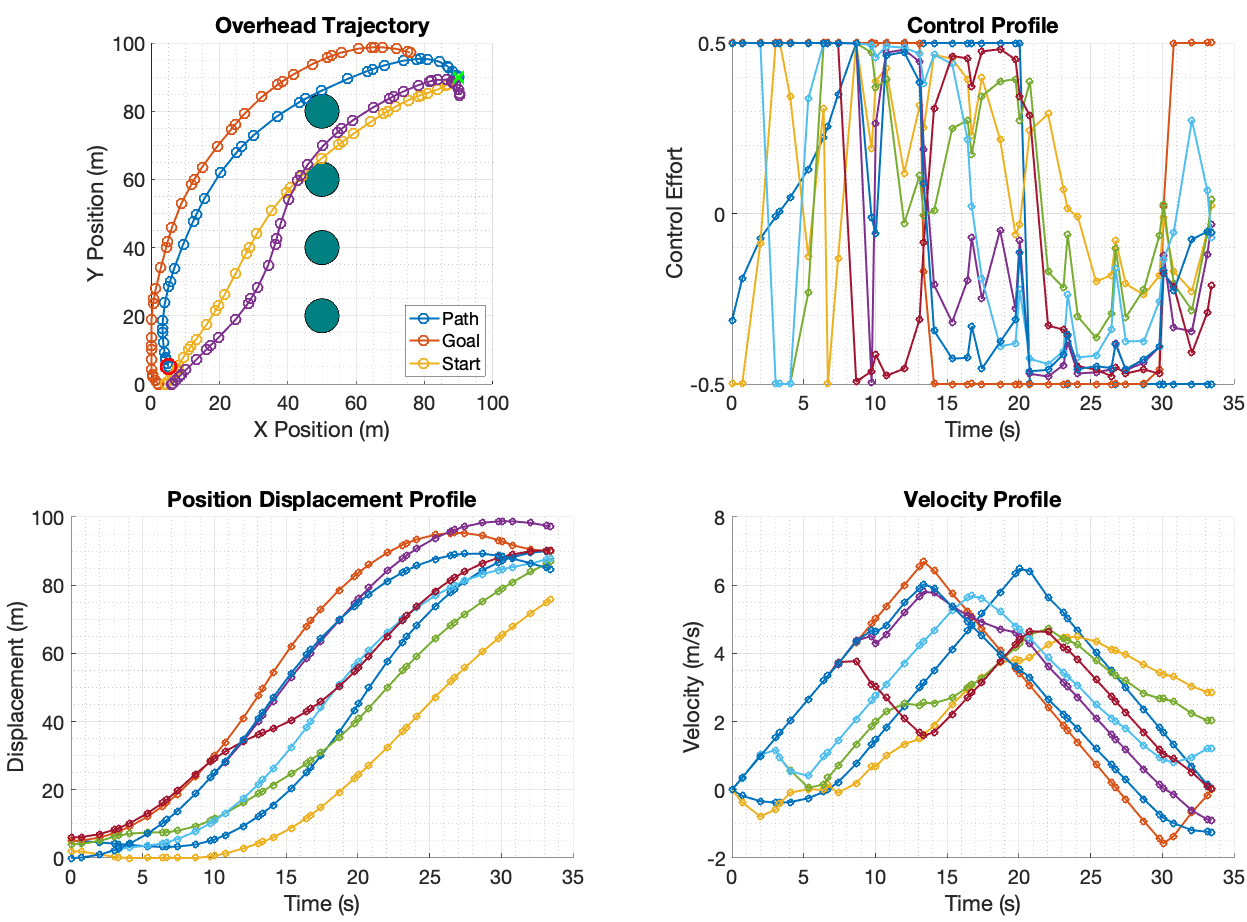
\includegraphics[width=0.75\textwidth]{img/results_1.png}
\caption{GPOPS-II optimal solution for four agents and four obstacles arranged vertically. The primary agent's position is highlighted in blue, in the plot on the top-left.}
\label{results_1}
\end{center}
\end{figure*}

\begin{figure*}[h!]
\begin{center}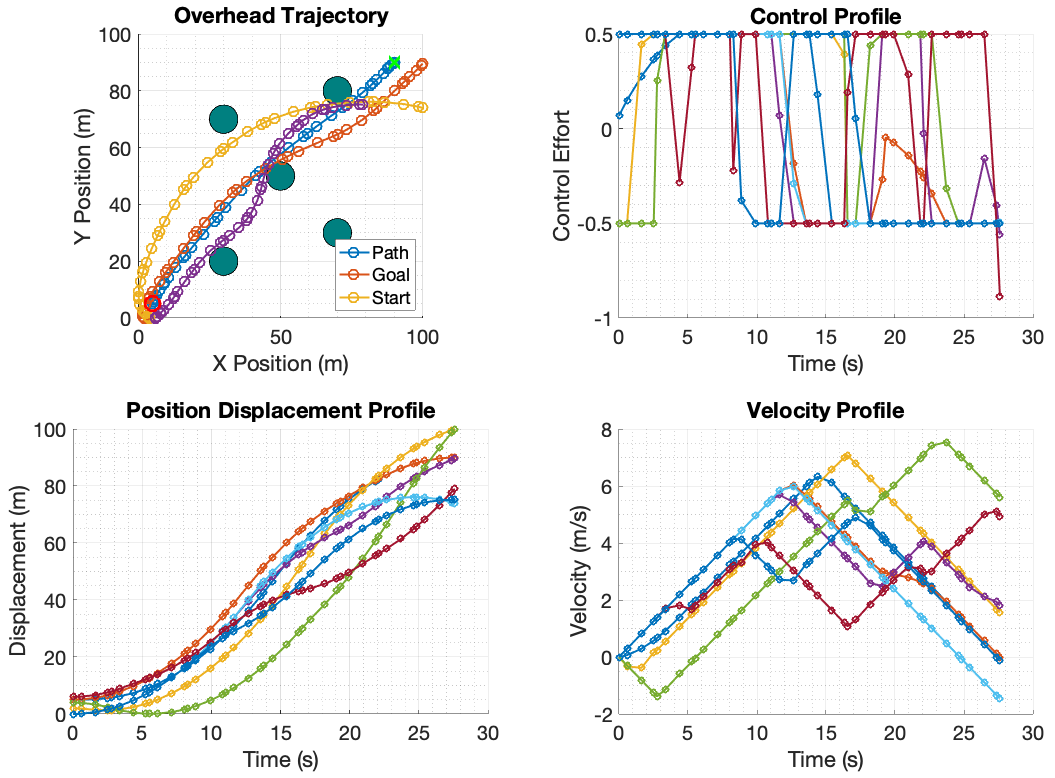
\includegraphics[width=0.75\textwidth]{img/results_2.png}
\caption{GPOPS-II optimal solution for four agents and five obstacles arranged in a cross pattern. The primary agent's position is highlighted in blue, in the plot on the top-left.}
\label{results_2}
\end{center}
\end{figure*}

% The results 

\section{Discussions}
The results show that it is possible to find (nearly-) optimal paths with a few numbers of agents and obstacles. Unfortunately, this technique scales poorly for larger problems.

On visual inspection, the results appear consistent with the qualitative features we expect: control profiles exhibit bang-bang behavior, agent paths are smooth, and secondary agents attempt to maximize the angular diversity to the primary agent. One interesting note is that the secondary agents do not "overtake" the agent to surround it completely, this may be the balance between the minimum-fuel and minimum GDOP objectives.

\section{Conclusions}
This report formulates and implements a centralized for maximizing the GDOP of a single agent in a multi-agent system. The problem was formulated as an optimization problem, which was solved numerically, using GPOPS-II.

GDOP is a single value which describes a complex phenomenon. As noted during the presentation of this project, a better metric would be to analyze the output of an estimator in real-time, which is the covariance matrix.

\subsection{Future Work}
A natural extension is to develop a controller that can be run in a decentralized manner. The centralized approach in this report would require complete communication to be implemented in an actual system.

Additionally, this problem assumes that the map is well-known. In real scenarios, it may only be possible to compute optimal solutions locally.

The agent dynamics in this report are relatively simple. This makes the solution and convergence more straightforward. It would be interesting to investigate complex dynamics, such as UAVs, ackermann-steered vehicles, or even legged robots.


\begin{thebibliography}{00}
\bibitem{florian} F. Meyer, H. Wymeersch, M. Fr\"{o}hle and F. Hlawatsch, "Distributed Estimation With Information-Seeking Control in Agent Networks," in IEEE Journal on Selected Areas in Communications, vol. 33, no. 11, pp. 2439-2456, Nov. 2015
\bibitem{spletzer} J. Spletzer, A. K. Das, R. Fierro, C. J. Taylor, V. Kumar and J. P. Ostrowski, "Cooperative localization and control for multi-robot manipulation," Proceedings 2001 IEEE/RSJ International Conference on Intelligent Robots and Systems. Expanding the Societal Role of Robotics in the Next illenium (Cat. No.01CH37180), Maui, HI, USA, 2001, pp. 631-636 vol .2
\bibitem{gdop}J. Zhu, "Calculation of geometric dilution of precision," in IEEE Transactions on Aerospace and Electronic Systems, vol. 28, no. 3, pp. 893-895, July 1992, doi: 10.1109/7.256323.
\bibitem{gpops}Patterson, M. A. and Rao, A. V., "GPOPS-II: A MATLAB Software for Solving Multiple-Phase Optimal Control Problems Using hp-Adaptive Gaussian Quadrature Collocation Methods and Sparse Nonlinear Programming", ACM Transactions on Mathematical Software, Vol. 41, No. 1., October 2014, pp. 1:1 - 1:37.

\end{thebibliography}

\end{document}
